\documentclass[twocolumn]{scrartcl}

\usepackage{fullpage}
\usepackage{graphicx}
\usepackage{float}
\usepackage[T1]{fontenc}

\usepackage[unicode=true,pdfusetitle,
bookmarks=true,bookmarksnumbered=false,bookmarksopen=false,
breaklinks=true,pdfborder={0 0 0},pdfborderstyle={},backref=false,colorlinks=true]
{hyperref}
\hypersetup{linkcolor=blue,citecolor=blue,urlcolor=blue}
\usepackage[backend=biber, maxbibnames=99, style=numeric, sorting=none]{biblatex}
\setlength\bibitemsep{2\itemsep}
\addbibresource{refs.bib}

%opening
\title{Report to the Guam Invasive Species Council on University of Guam Invasive Species Activities}
\author{Aubrey Moore}

\begin{document}

\maketitle

\section{Pacific Ecological Security Conference (PESC)}

The PESC, held in Palau during October 2022, brought together island leaders, development partners, regional organizations, agricultural/food security and natural resource managers, and the media to discuss the importance of managing and preventing the spread of invasive species in Pacific Island environments \cite{anonymousFirstPacificEcological2022}.

 Conference hosts and sponsors included Government of Palau Ministry of Agriculture, Fisheries, and Environment, Secretariat of the Pacific Community (SPC), the East-West Center, the Global Environment Facility (GEF), the Nature Conservancy, the US Department of the Interior - Office of Insular Affairs, the U.S. Forest Service, and the Ocean Policy Research Institute.

Delegates from Guam were Roland Quitugua and Aubrey Moore from UOG and Glenn Dulla and Andrea Blas from the Department of Agriculture. The Guam delegation participated in a satellite meeting organized by the U.S. Department of the Interior - Office of Insular Affairs and the U.S. Forest Service. At this meeting each island group presented a status report on invasive species issue (See \parencite{mooreOverviewInvasiveSpecies2022-10-06} for slides from the Guam presentation). This was followed by discussions on federal funding and collaboration.  

\subsection{Strategic Action Plan for Coconut Rhinoceros Beetle (CRB)}

Prior to the PESC, members of the Guam delegation worked with colleagues throughout the Pacific to write a Pacific-wide strategic action plan for response to the recent spread of CRB. This plan was accepted by PESC delegates and has been published online \cite{conferenceStrategicActionPlan2022}.

The plan includes five objectives:

\begin{enumerate}
	\item Enhance Regional Coordination and support of PICTs to achieve the
	objectives of the CRB Strategic Action Plan (SAP)
	\item Conduct immediate and long-term collaborative research to develop
	tools and understanding necessary to enable effective CRB prevention, control, and
	eradication
	\item Prevent the spread of CRB to new locations in the Pacific region and
	beyond
	\item Implement an active early detection, and rapid response system for new
	outbreaks at regional and island levels
	\item Improve implementation of control efforts and mitigate the impacts of
	CRB where already present in the region
	
\end{enumerate} 

\section{Recently Detected Invasive Species}

\subsection{Citrus blackfly, \textit{Aleurocanthus woglumi}}

This major pest of citrus was first detected on Guam in March 2023 \cite{moore2023}. It is not expected to cause major damage because it is parasitized by biological control agents previously introduced for a closely related insect pest, the orange spiny whitefly, \textit{A. spiniferus}.

\begin{figure}[H]
	\centering
	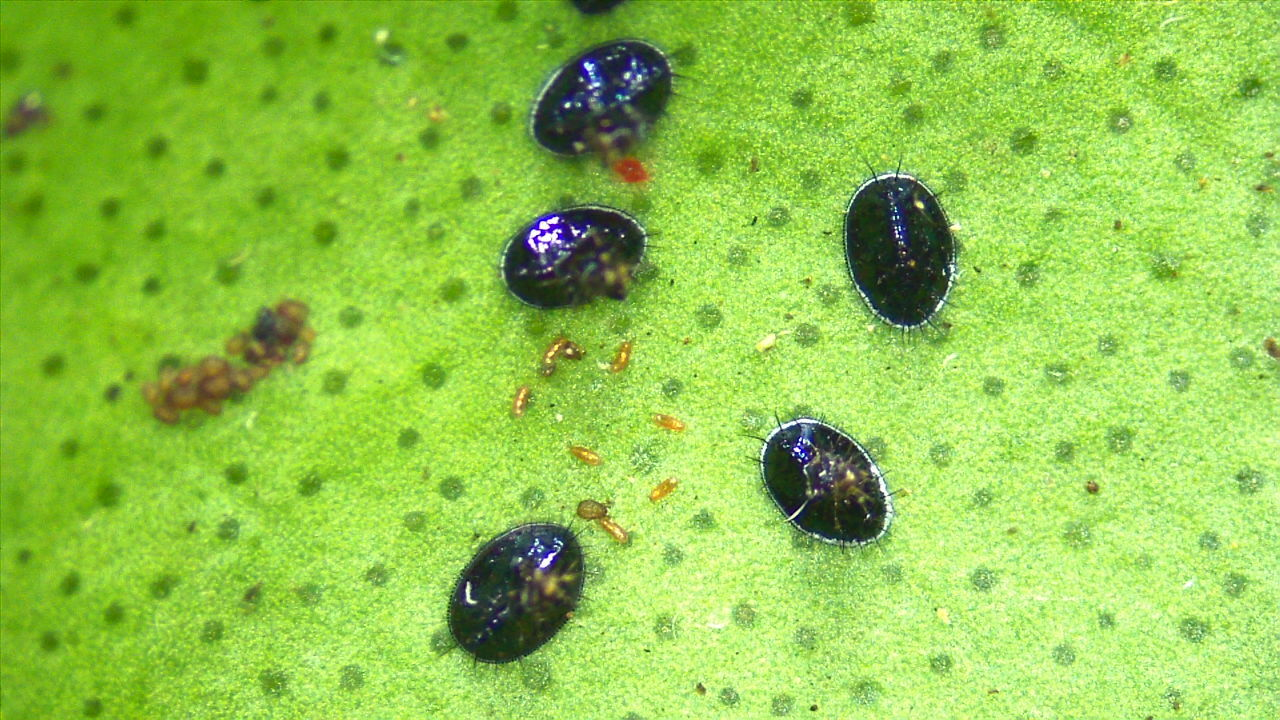
\includegraphics[width=\linewidth]{images/woglumi}
	\caption{Citrus blackfly, \textit{Aleurocanthus woglumi}}
	\label{fig:woglumi}
\end{figure}


\section{Work on Coconut Rhinoceros Beetle (CRB)}

\subsection{Island-wide CRB Damage Survey}

An island-wide CRB damage survey is performed every few moths by taking images of trees growing along the sides of all major roads on Guam at a rate of one image per second. Each image is run through an artificial intelligence program which finds all coconut palms and assigns a damage rating to each one. Results are returned as an online interactive map. In the latest survey, done in April 2023, one in five (20\%) of Guam's coconut palms growing along roadsides were damaged by CRB \cite{moorePressRelease2023} (Fig, \ref{fig:timeline}).

% TODO: \usepackage{graphicx} required
\begin{figure}[H]
	\centering
	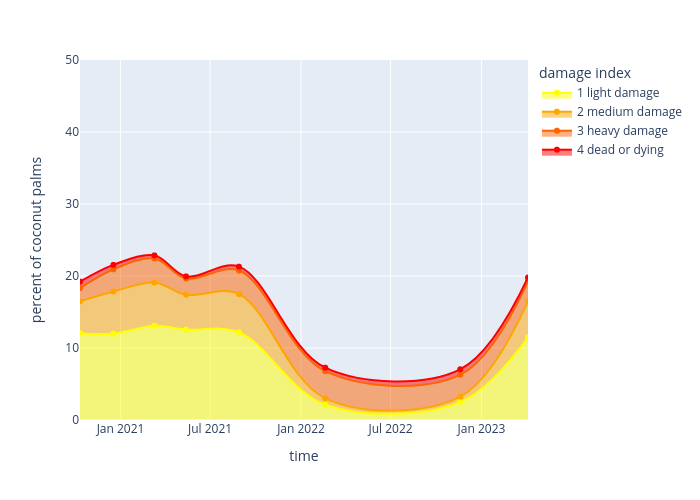
\includegraphics[width=1\linewidth]{images/timeline}
	\caption{Percent of coconut palms growing along Guam's roadsides which show visible damage from coconut rhinoceros beetle.}
	\label{fig:timeline}
\end{figure}

\subsection{CRB Biological Control}

UOG is participating in a Pacific-wide effort to find an effective biological control agent for CRB-G, the rhino beetle biotype which was first discovered on Guam. This biotype has also invaded Rota, Hawaii, Papua New Guinea, Solomon Islands. It is causing massive damage on these islands and is likely to spread further if infestations are not brought under control. Entomologists are searching for an isolate of a virus called \textit{Oryctes rhinoceros} nudivirus (OrNV) which infects rhino beetles and stops them from reproducing.

OrNV samples from Palau were recently tested but no significant responses were detected. The next set of isolates to be screened are from the Philippines.

This work is being done in collaboration with the Tokyo University of Agriculture and Technology, Palau Community College, and AgResearch New Zealand \cite{hansonUOGTokyoUniversity}. This work is funded by grants from DOI-OIA and the US Forest Service.

\clearpage

\section{Work on Cycad Aulacaspis Scale (CAS)}

Cycad Aulacaspis scale insect (CAS), detected in 2003, has killed most of Guam’s endemic cycads, \textit{Cycas micronesica}. This plant went from being the
most abundant tree in Guam’s forests in 2002 to being placed on the US endangered species list in 2015. Annual surveys of 12 permanent forest
plots indicate that only 4\% of the original \textit{C. micronesica} survive and no reproduction is taking place. All seeds and seedlings are currently being killed by CAS and other invasive species, making restoration unfeasible. 

Work towards finding effective biological control agents for CAS continues \cite{caveBiologicalControlCycad2022}. In March 2022, UOG hosted a visit to Guam by Dr. Ronald Cave, a CAS biocontrol expert from the University of Florida \cite{caveBiologicalControlCycad2022a}. Following his trip, Dr. Cave provided recommendations for responding to CAS \cite{caveReportUSFish2022}. This prompted an \textit{ad hoc} cycad scale working group organized by the US Fish and Wildlife service which holds frequent online meetings. Three grant proposals have recently been submitted by members of this group.

\section{Miscellaneous}

\begin{itemize}
	\item A new program entitled \textit{Plant Protection and Biosecurity for Guam and Micronesia} was submitted to the National Institute of Food and Agriculture. This program has been approved but not yet funded \cite{NIFA2022}.

	\item Two UOG programs, the Guam Plant Extinction Prevention Program (GPEPP) and the Center for Island Sustainability (CIS) and are propagating \textit{Cycas micronesica} are conducting field studies which include monitoring and controlling invasive species. 
	
	\item UOG has recently hired Dr. Glenn Dulla as a plant pathologist and Dr. Rachel Jolly as a restoration ecologist.
\end{itemize}


\clearpage
\printbibliography

\end{document}
